\chapter{映像伝送システム}
\label{chap:video-transmission}

\section{ビデオカメラ}



\section{ディスプレイ}



\section{インターレース}



\section{色空間}

一般的に液晶ディスプレイでは、1ピクセルを赤、緑、青、すなわちRGBの3つの色信号で表現する。
多くのPCやゲーム機の出力では、RGBそれぞれに8bitで表現するため、1ピクセルあたり24bitとなり、16,777,216色を表現することができる。

一方、ビデオカメラの出力では、輝度信号Yと、2つの色差信号を使って表現される色空間であるYUVが用いられることが多い。
この方式の特徴は、「人間の目は明るさの変化には敏感だが、色の変化には鈍感である」という性質に基づいて、色度信号の情報量を減らすことができるという点にある。
YUV 4:2:2では、輝度信号は1ピクセル毎、色差信号は2ピクセル毎にある。これにより、帯域を1/2に減らすことが可能である。
また、YUV 4:2:0では、輝度信号は1ピクセル毎、色差信号は4ピクセル毎になる。これにより、帯域を1/4に減らすことが可能である。

\begin{figure}[htbp]
    \begin{center}
        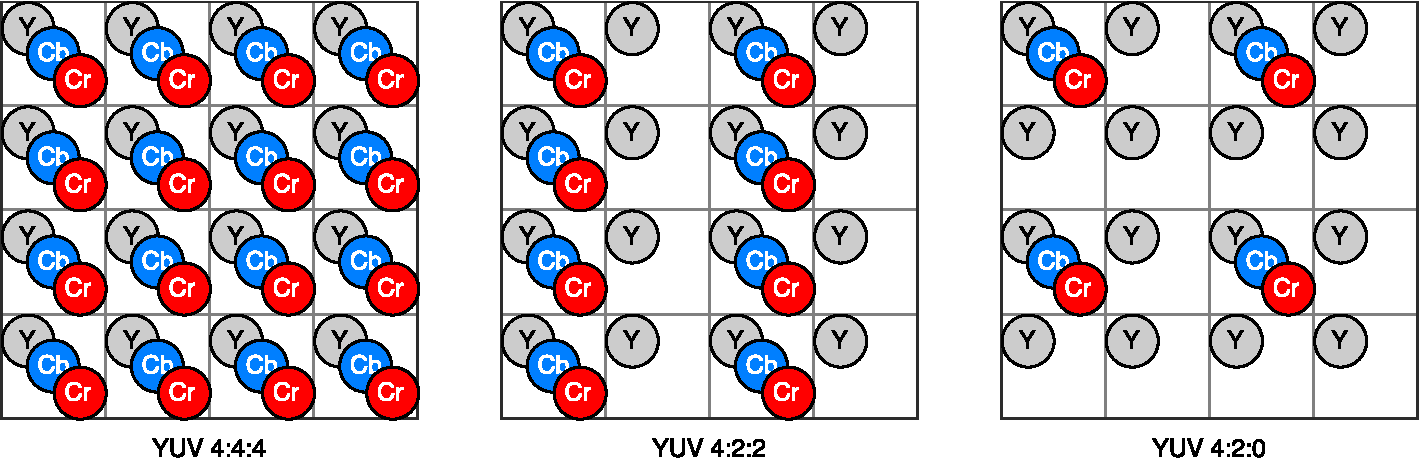
\includegraphics[bb=0 0 681 222,width=15.5cm]{img/yuv-pixel-structure.pdf}
    \end{center}
    \caption{Implement Flow}
    \label{fig:yuv-pixel-structure}
\end{figure}

HDMIで用いられる、YCbCrでは、
また、複数ピクセル

YCbCr

映像では一般的に、RGBやYUV, YCbCr, YPbPrといった色空間で表現される。
色差成分を間引くことにより、

\section{帯域}

帯域は次のようになる。

表は次のように出力される。(表\ref{tb:video-bandwidth})

\begin{table}[htbp]
  \caption{解像度、フレームレート、色空間による帯域の変化}
  \label{tb:video-bandwidth}
  \begin{center}
  \begin{tabular}{c|c|c|c|c}
    \hline
    解像度     & フレームレート & 色空間 & ピクセルあたりのビット数 & 帯域\\\hline\hline
    3840x2160 & 60P          & RGB    & X bit               & XX Gbps\\\hline
    3840x2160 & 30P          & RGB    & X bit               & XX Gbps\\\hline
    3840x2160 & 30P          & RGB    & X bit               & XX Gbps\\\hline
    3840x2160 & 30P          & YUV444 & X bit               & XX Gbps\\\hline
    3840x2160 & 30P          & YUV422 & X bit               & XX Gbps\\\hline
    3840x2160 & 30P          & YUV420 & X bit               & XX Gbps\\\hline
    1920x1080 & 60P          & RGB    & X bit               & XX Gbps\\\hline
    1920x1080 & 60P          & YUV    & X bit               & XX Gbps\\\hline
    1920x1080 & 30P          & RGB    & X bit               & XX Gbps\\\hline
  \end{tabular}\end{center}
\end{table}

\section{インターフェース}
\subsection{HDMI 1.4/2.0}

% \begin{table}[htbp]
%   \caption{解像度、フレームレート、色空間による帯域の変化}
%   \label{tb:hdmi-feature}
%   \begin{center}
%   \begin{tabular}{c|c|c|c|c}
%     \hline
%               & HDMI 1.4 & HDMI 2.0 \\\hline\hline
%     3840x2160 & 60P          & RGB    & X bit               & XX Gbps\\\hline
%     3840x2160 & 30P          & RGB    & X bit               & XX Gbps\\\hline
%     3840x2160 & 30P          & RGB    & X bit               & XX Gbps\\\hline
%     3840x2160 & 30P          & YUV444 & X bit               & XX Gbps\\\hline
%     3840x2160 & 30P          & YUV422 & X bit               & XX Gbps\\\hline
%     3840x2160 & 30P          & YUV420 & X bit               & XX Gbps\\\hline
%     1920x1080 & 60P          & RGB    & X bit               & XX Gbps\\\hline
%     1920x1080 & 60P          & YUV    & X bit               & XX Gbps\\\hline
%     1920x1080 & 30P          & RGB    & X bit               & XX Gbps\\\hline
%   \end{tabular}\end{center}
% \end{table}

\section{伝送手法}

\section{まとめ}
